\chapter{Puesta en marcha del equipo}

\section{Introducción}

El presente documento describe el desarrollo y las funcionalidades de un equipo diseñado para el proyecto Acuacol, el cual tiene como objetivo optimizar y automatizar los procesos involucrados en un sistema de acuaponía. Este tipo de sistema combina la cría de peces con el cultivo de plantas en un entorno controlado, donde la correcta monitorización y gestión de variables tanto del agua como del ambiente es crucial para el éxito del ecosistema.

El equipo desarrollado dentro del marco del proyecto es capaz de monitorizar y registrar una serie de parámetros fundamentales para el funcionamiento de un sistema de acuaponía. Entre las funcionalidades del equipo destacan la medición de la temperatura y la humedad del aire en dos puntos distintos, así como la temperatura del agua en dos zonas específicas. Adicionalmente, se incluye la medición de variables críticas como el pH del agua, la conductividad eléctrica y la concentración de oxígeno disuelto en el agua.

Además de la monitorización, el equipo cuenta con dos entradas digitales diseñadas para conectarse a interruptores de boya, lo que permitiría una supervisión automatizada del nivel de los depósitos de agua. Asimismo, el hardware incorpora dos salidas por relé, que están destinadas a controlar una electroválvula para la gestión del nivel de un depósito y una bomba dosificadora que ajusta el pH del agua. Aunque estas funcionalidades de control aún no están operativas en esta versión del software, el equipo ha sido diseñado para soportarlas en futuras actualizaciones.

El equipo realiza un muestreo de todas estas variables cada 5 segundos, almacenando los datos recogidos en una tarjeta microSD para su posterior análisis cada 15 minutos. Además, estos datos se suben a la nube, lo que permite una supervisión remota y facilita la toma de decisiones en tiempo real sobre el sistema acuapónico.

Este sistema, por tanto, representa un avance significativo en la automatización de los procesos de acuaponía, proporcionando una base sólida para mejorar la eficiencia y sostenibilidad de estos sistemas en entornos de producción agrícola y acuícola.

\newpage

\section {Hardware}

Vamos a empezar describiendo las conexiones del equipo e iremos viendo cada sensor por separado.

\begin{figure}[htbp!]
\centering{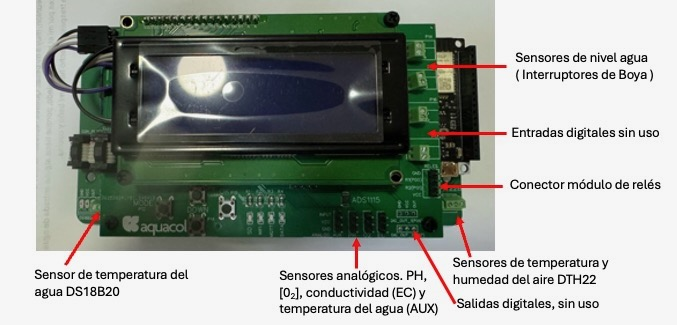
\psfig{file=Figuras/Montaje_Arriba.jpeg,width=16cm,angle=0}}
\caption{Placa montada Acuacol}\label{placa:acuacol}
\end{figure}

%%%%%%%%%%%%%%%%%%%%%%%%%%%%%%%%%%%%%%%%%%%%%
%                   relés                   %
%%%%%%%%%%%%%%%%%%%%%%%%%%%%%%%%%%%%%%%%%%%%%

En esta versión del Hardware de Acuacol \underline{no se usarán los sensores de nivel del agua ni el} \underline{módulo de relés}. Las conexiones están hechas de modo que cuando se crea conveniente puedan ser usadas. En la caja proporcionada deberían venir los módulos de relés.

\begin{figure}[htbp!]
\centering{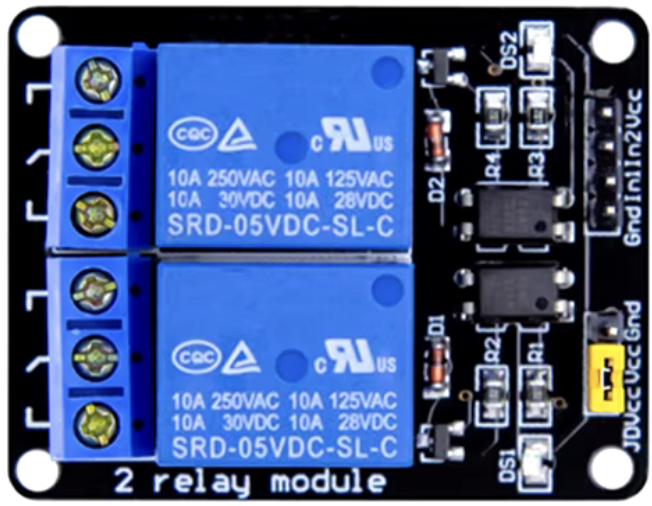
\psfig{file=Figuras/Modulo_reles.png,width=7cm,angle=0}}
\caption{Modulo de relés}\label{modulo:reles}
\end{figure}

Conexionado 
\begin{itemize}
\item El terminal \emph{GND} del módulo de relés se conecta al \emph{GND} del conector de relés de la placa.
\item El terminal \emph{VCC} del módulo de relés se conecta al \emph{VCC} del conector de relés de la placa.
\item El terminal \emph{IN1} del módulo de relés se conecta al \emph{R1(P00)} del conector de relés de la placa.
\item El terminal \emph{IN2} del módulo de relés se conecta al \emph{R2(P01)} del conector de relés de la placa.
\end{itemize}

P00 y P01 hacen referencia a la dirección de esos pines a nivel de programación.

%%%%%%%%%%%%%%%%%%%%%%%%%%%%%%%%%%%%%%%%%%%%%
%                   DTH22                   %
%%%%%%%%%%%%%%%%%%%%%%%%%%%%%%%%%%%%%%%%%%%%%

\subsection{Sensores de temperatura y humedad del aire DTH22}

Los sensores DTH22 no vienen conectados. Se conectan en la parte derecha de la placa inferior:

\begin{figure}[htbp!]
\centering{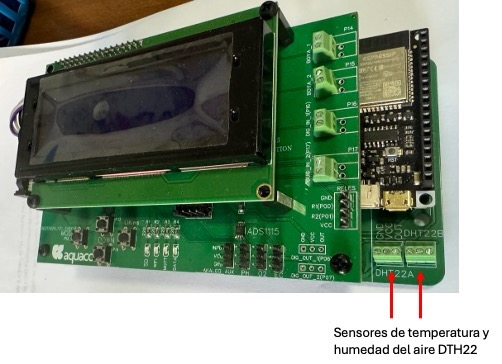
\psfig{file=Figuras/Montaje_derecha.jpeg,width=10cm,angle=0}}
\caption{Conexión en la placa del DTH22}\label{placa:acuacol:derecha}
\end{figure}

En la figura \ref{placa:acuacol:derecha} se pueden observar dos bornes para conectar dos sensores DTH22. La idea es que el sensor DTH22 conectado al borne "DTH22A" mida la temperatura y la humedad del aire en el interior de la sala donde se encuentran los depósitos de los peces. El sensor DTH22 conectado al borne "DTH22B" medirá la temperatura y la humedad del aire exterior. Para ello, este sensor debe instalarse en el exterior, asegurándose de que esté protegido del agua. Será necesario soldar un cable al sensor para esta instalación. El cable debe ser de al menos 3 hilos, apantallado, y no importa demasiado la sección del mismo. La longitud debe ser la mínima posible, ya que, aunque el protocolo de comunicaciones que utiliza el DTH22 permite cables bastante largos (20m según la literatura), el sensor funciona mejor con cables cortos.

\begin{figure}[htbp!]
\centering{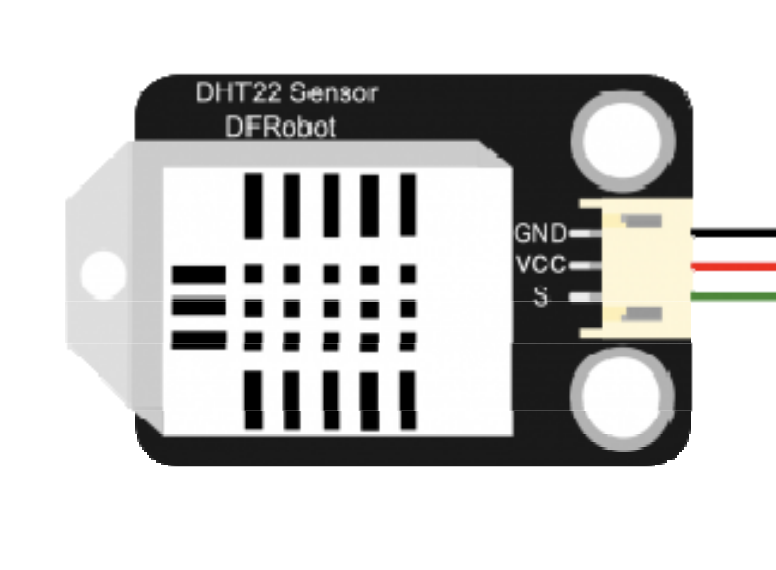
\psfig{file=Figuras/DTH22.png,width=10cm,angle=0}}
\caption{Conexion DTH22}\label{modulo:dth22}
\end{figure}

\begin{itemize}
\item El terminal \emph{GND} del DTH22 se conecta al \emph{GND} del borne "DTH22" de la placa.
\item El terminal \emph{VCC} del DTH22 se conecta al \emph{VCC} del borne "DTH22" de la placa.
\item El terminal \emph{S} del DTH22 se conecta al \emph{OUT} del borne "DTH22" de la placa.
\end{itemize}

Si la instalación es abierta, ambos sensores miden lo mismo. Solo se conectaría uno de los dos.

\begin{tcolorbox}
[colback=red!5!white,colframe=red!75!black,fonttitle=\bfseries,title=Desmontaje ]
Sea cuidadoso con el conexionado. Durante las pruebas del hardware se han pasado los tornillos con facilidad. Por eso, se recomienda el desmontaje de las placas para hacer las conexiones de forma más sencilla.
\begin{enumerate}
\item Quite los 4 tornillos de teflón del LCD (suelen ser solo 2). El LCD quedará unido a la placa de arriba por 4 hilos (figura \ref{desmontaje:1}).
\item Quite los 2 tornillos y los 2 separadores marcados en la figura \ref{desmontaje:2}. Quedará la placa de arriba suelta, conectada por un cable de 6 hilos a la placa inferior y por los 4 cables de los sensores analógicos. Puede quitar el conector de 6 hilos de la placa de arriba con la de abajo puesto que no tiene posibilidad de error al volverlo a montar. Puede quitarlos los cables de los sensores analógicos si tiene claro como van conectados. No quite los separadores de la parte inferior de la placa de arriba.
\item La placa inferior va unida a la caja con 2 tornillos metálicos (figura \ref{desmontaje:3}). Si los quita puede retirar la placa y hacer las conexiones cómodamente. Recuerde pasar los cables por el prensaestopa (pasacables) antes de hacer las conexiones. 
\item Para montar siga los pasos al contrario.
\end{enumerate}
\end{tcolorbox}

\begin{figure}[htbp!]
\centering{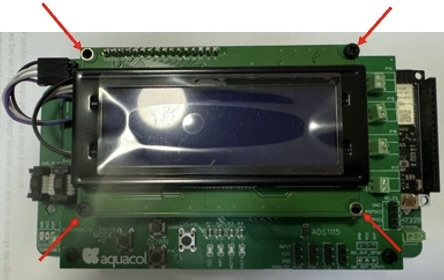
\psfig{file=Figuras/desmontaje1.jpeg,width=9cm,angle=0}}
\caption{Tornillos del modulo lcd.}\label{desmontaje:1}
\end{figure}

\begin{figure}[htbp!]
\centering{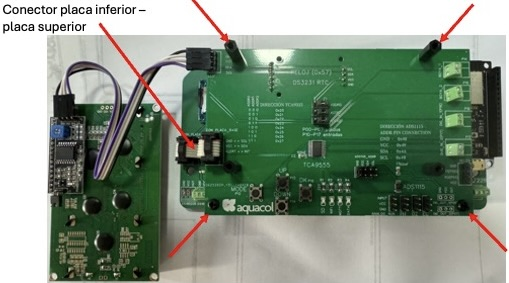
\psfig{file=Figuras/desmontaje2.jpeg,width=12cm,angle=0}}
\caption{Tornillos placa superior.}\label{desmontaje:2}
\end{figure}

\begin{figure}[htbp!]
\centering{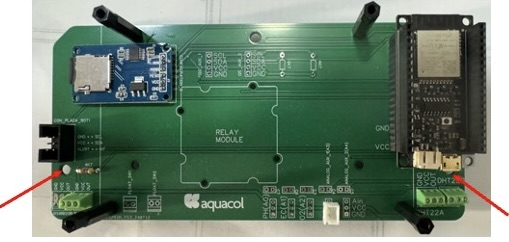
\psfig{file=Figuras/desmontaje3.jpeg,width=9cm,angle=0}}
\caption{Tornillos metálicos de placa inferior.}\label{desmontaje:3}
\end{figure}

%%%%%%%%%%%%%%%%%%%%%%%%%%%%%%%%%%%%%%%%%%%%%
%                   DS10B20                 %
%%%%%%%%%%%%%%%%%%%%%%%%%%%%%%%%%%%%%%%%%%%%%

\subsection{Sensor de temperatura del agua DS18B20}

El sensor DS1820 tampoco viene conectado. Se conectan en la parte izquierda de la placa inferior:

\begin{figure}[htbp!]
\centering{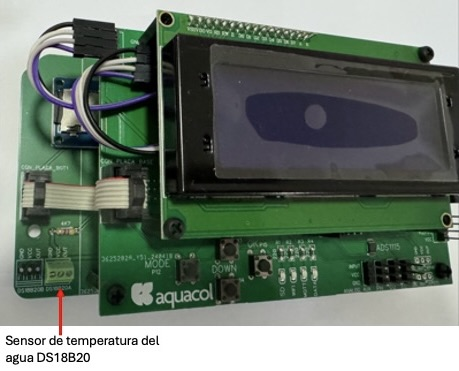
\psfig{file=Figuras/Montaje_DS18B20.jpg,width=10cm,angle=0}}
\caption{Conexión en la placa del DS18B20}\label{placa:acuacol:ds18b20}
\end{figure}

En la figura \ref{placa:acuacol:ds18b20} se observa que solo uno de los dos posibles bornes está soldado a la placa. Esto se debe a que, inicialmente, el equipo tenía dos sensores DS18B20, pero posteriormente se reemplazó uno de ellos por el sensor de temperatura incorporado en la sonda de conductividad. El objetivo es que este sensor mida la temperatura de un segundo tanque o piscina. Además, se utilizará esta sonda para calibrar el sensor de concentración de oxígeno ($O_2$) en caso de que se decida realizar la calibración con agua saturada. Esto se detallará en el apartado correspondiente (referencia pendiente).

\begin{figure}[htbp!] 
\centering{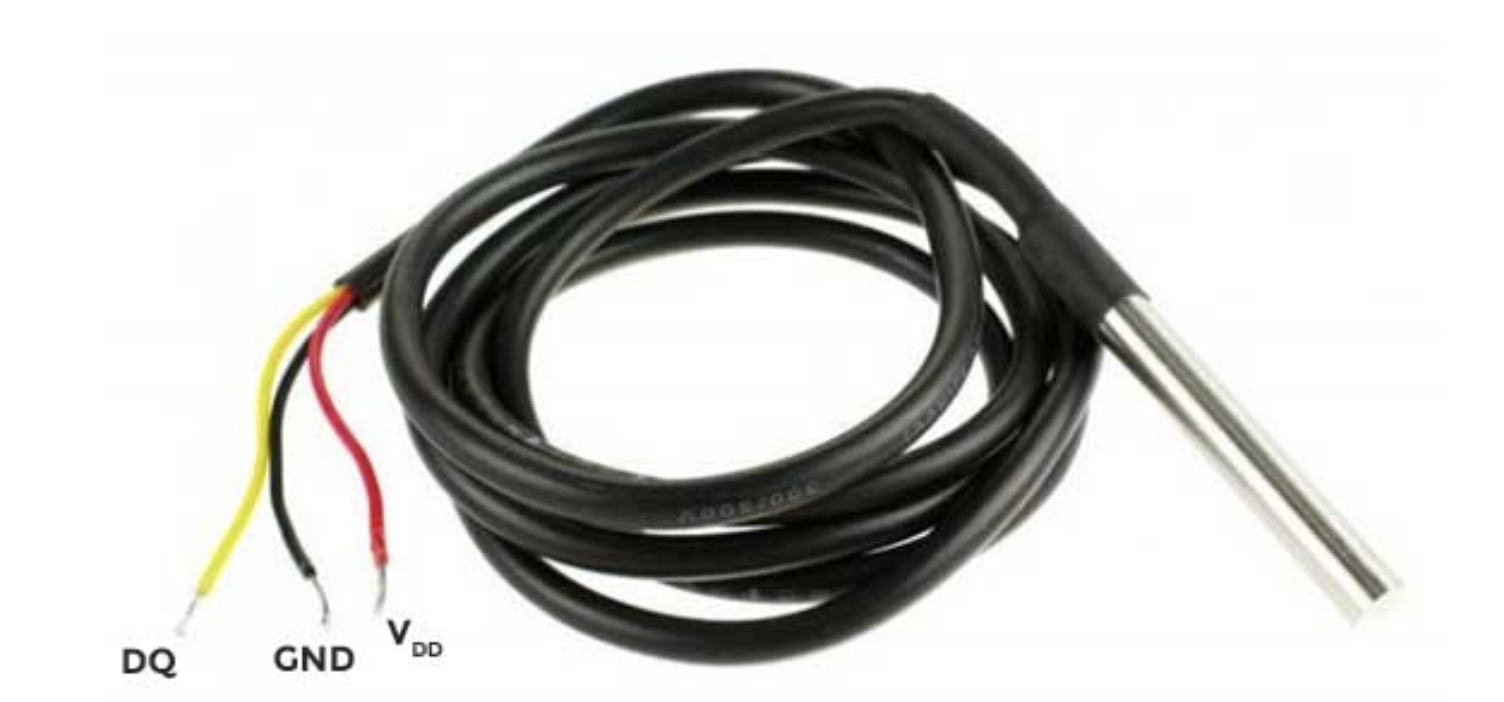
\psfig{file=Figuras/DS18B20.png,width=10cm,angle=0}} 
\caption{Sensor de temperatura del agua DS18B20}\label{sensor:ds18b20} 
\end{figure}

Las conexiones del DS18B20 se realizan de la siguiente manera:

\begin{itemize} 
\item El terminal \emph{GND} (negro) del DS18B20 se conecta al \emph{GND} del borne "DS18B20A" de la placa. 
\item El terminal \emph{VCC} (rojo) del DS18B20 se conecta al \emph{VCC} del borne "DS18B20A" de la placa. 
\item El terminal \emph{DQ} (amarillo) del DS18B20 se conecta al \emph{OUT} del borne "DS18B20A" de la placa. 
\end{itemize}

Se recomienda utilizar el propio cable que trae la sonda. Si el cable es demasiado corto, se puede extender con un cable de 3 hilos apantallado, similar al que trae el sensor. Es preferible mantener el cable lo más corto posible. Aunque la literatura indica que el protocolo 1-Wire, que utiliza el DS18B20, admite longitudes de cable de hasta 200 metros, algunos autores sugieren no exceder los 8 metros. Para evitar la corrupción de la señal, se ha añadido una resistencia PULLUP de 4.7 $k\Omega$.

\subsection{Sensores analógicos}

Los sensores analógicos son aquellos que me dan la medida en forma de tensión. Son muy sensibles a interferencias y se deben poner lo más cerca posible del equipo. Como todos estos sensores se ponen juntos en el baño donde se hallen los peces , el equipo habría de situarse lo más cerca posible de este baño.

Estos sensores son:
\begin{itemize}
\item \textbf{Sensor de PH DFRobot SEN0169-V2}. El transductor (la placa que adapta la señal de la sonda para que pueda ser leída por el microcontrolador) del sensor de pH ya viene conectado, por lo que solo es necesario conectar la sonda de pH al conector en el exterior del equipo.  
\begin{figure}[htbp!] 
\centering{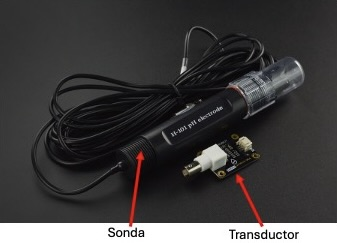
\psfig{file=Figuras/PH.jpg,width=10cm,angle=0}} 
\caption{Sensor de PH DFRobot SEN0169-V2}\label{sensor:PH} 
\end{figure}
Se puede observar que el transductor del sensor de pH está unido a otra placa, la DFRobot DFR0504, que es un aislador analógico (ANALOG ISOLATOR) (figura \ref{sensor:iso}). Este aislador se utiliza para evitar el acoplamiento entre las diferentes señales analógicas a través del agua.
\begin{figure}[htbp!] 
\centering{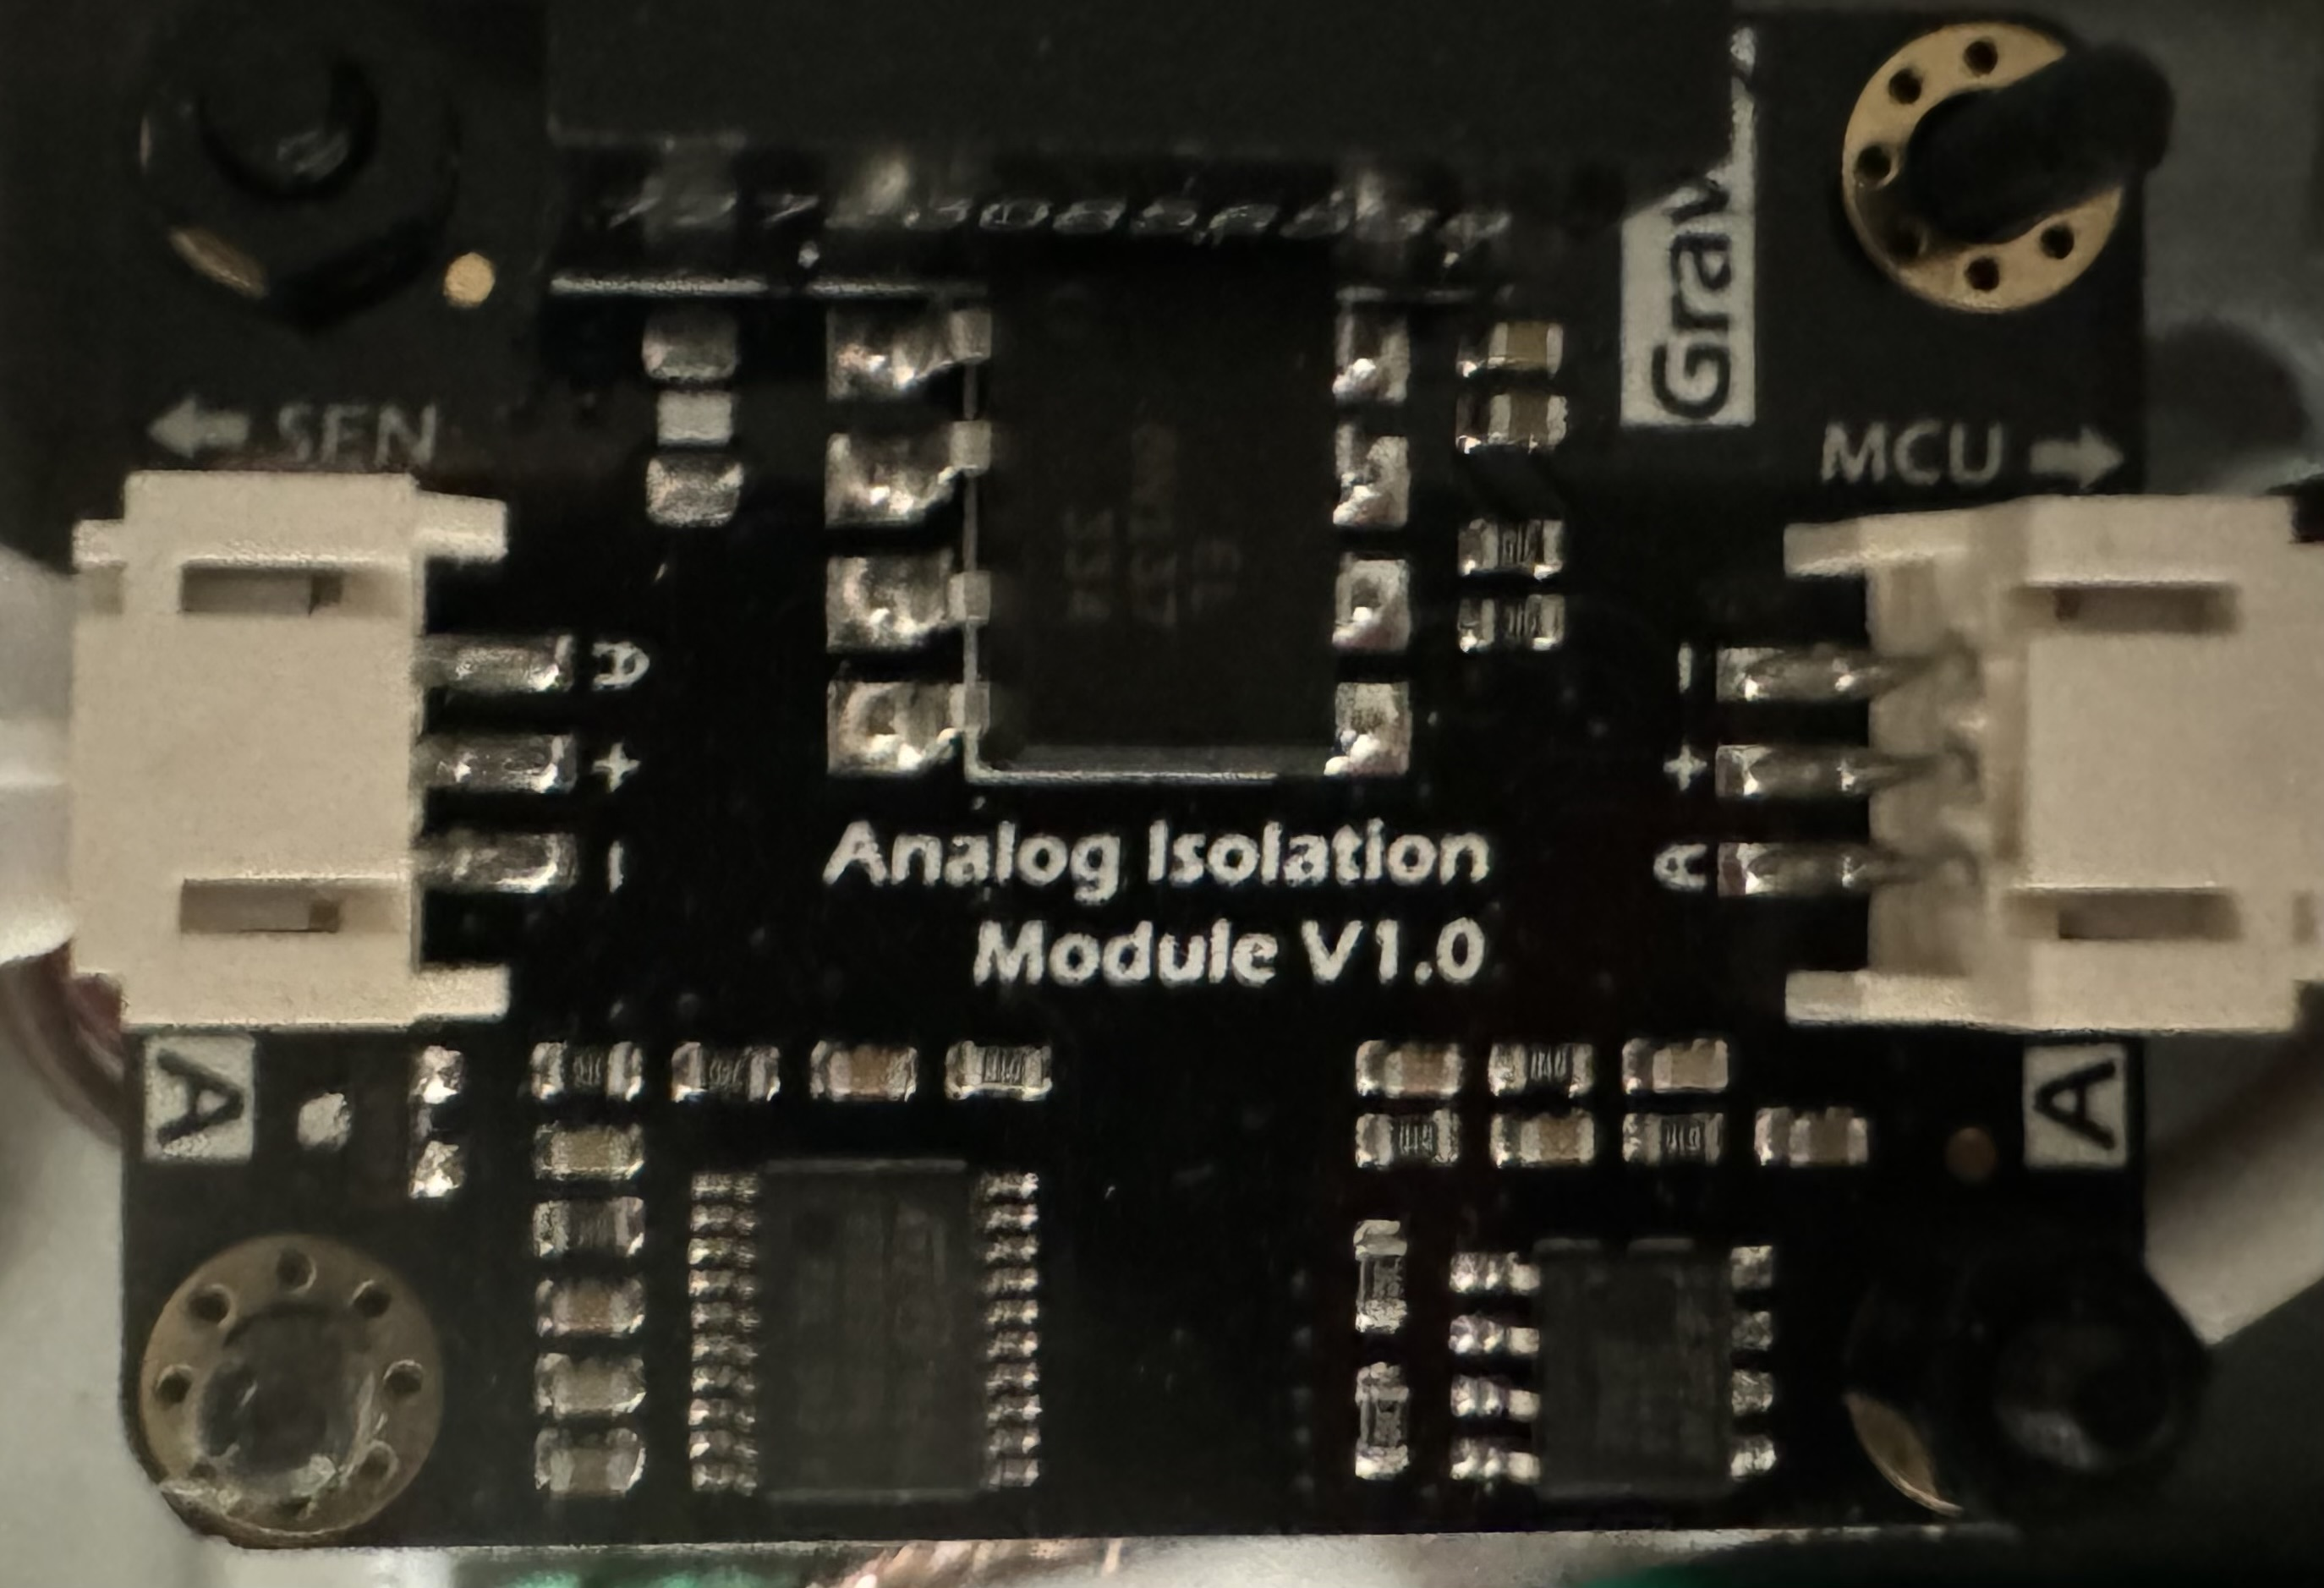
\psfig{file=Figuras/Analog_isolator.jpeg,width=8cm,angle=0}} 
\caption{Analog isolator}\label{sensor:iso} 
\end{figure}

Lo mismo ocurre con los transductores del sensor de 02 y del de conductividad.

\item \textbf{El sensor de concentración de oxígeno DFRobot SEN0237-A}. El transductor ya está conectado, solo hay que poner la sonda de $O_2$ en el conector en el exterior del equipo. 
\begin{figure}[htbp!] 
\centering{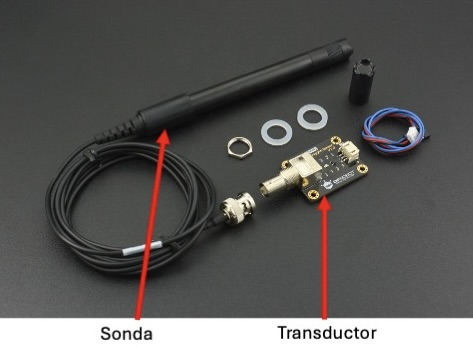
\psfig{file=Figuras/O2.jpg,width=10cm,angle=0}} 
\caption{Sensor de O2 DFRobot SEN0237-A}\label{sensor:O2} 
\end{figure}

\item El sensor de conductividad y temperatura (DFRobot SEN0451). los transductores (las placas que adaptan las señales de la sonda para que las pueda leer el micro) vienen apilados uno sobre otro en la parte inferior izquierda de la caja ya vienen conectados. Se puede observar que vienen sueltos, es porque hay que poner los conectores correspondientes a la sonda de conductividad y temperatura (figura \ref{sensor:EC}, Conector transductor -sensor). Estos conectores no entran por el agujero del prensaestopa (pasacables) negro que está atornillado en la parte inferior de la caja. 
\begin{figure}[htbp!] 
\centering{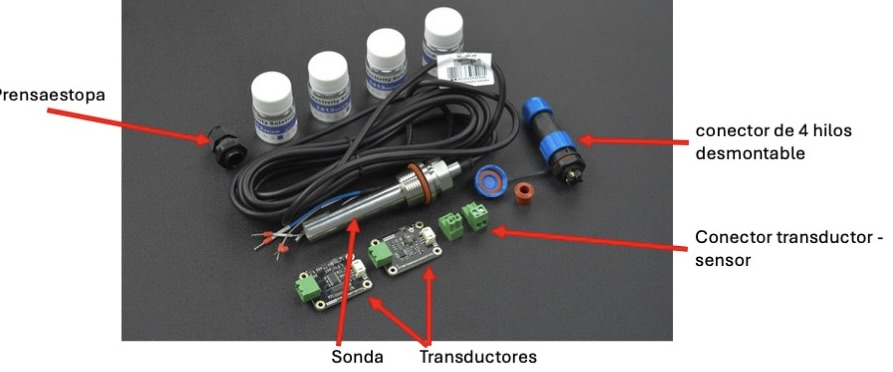
\psfig{file=Figuras/EC.jpg,width=14cm,angle=0}} 
\caption{Sensor de EC DFRobot SEN0451}\label{sensor:EC} 
\end{figure}

Por lo que se procederá de la siguiente manera:
\begin{enumerate}
\item Pasamos el cable (figura \ref{sensor:CEC}) de la sonda por el prensaestopa de color negro (que ya está puesto en la caja).
\item Conectamos los cables a los conectores transductor-sensor (ver figura \ref{sensor:EC}). En una de las fichas verdes se conectan los dos cables marcados con \emph{temp} (figura \ref{sensor:CEC}). No importa el orden (figura \ref{sensor:temp}).\\ 
\begin{figure}[htbp!] 
\centering{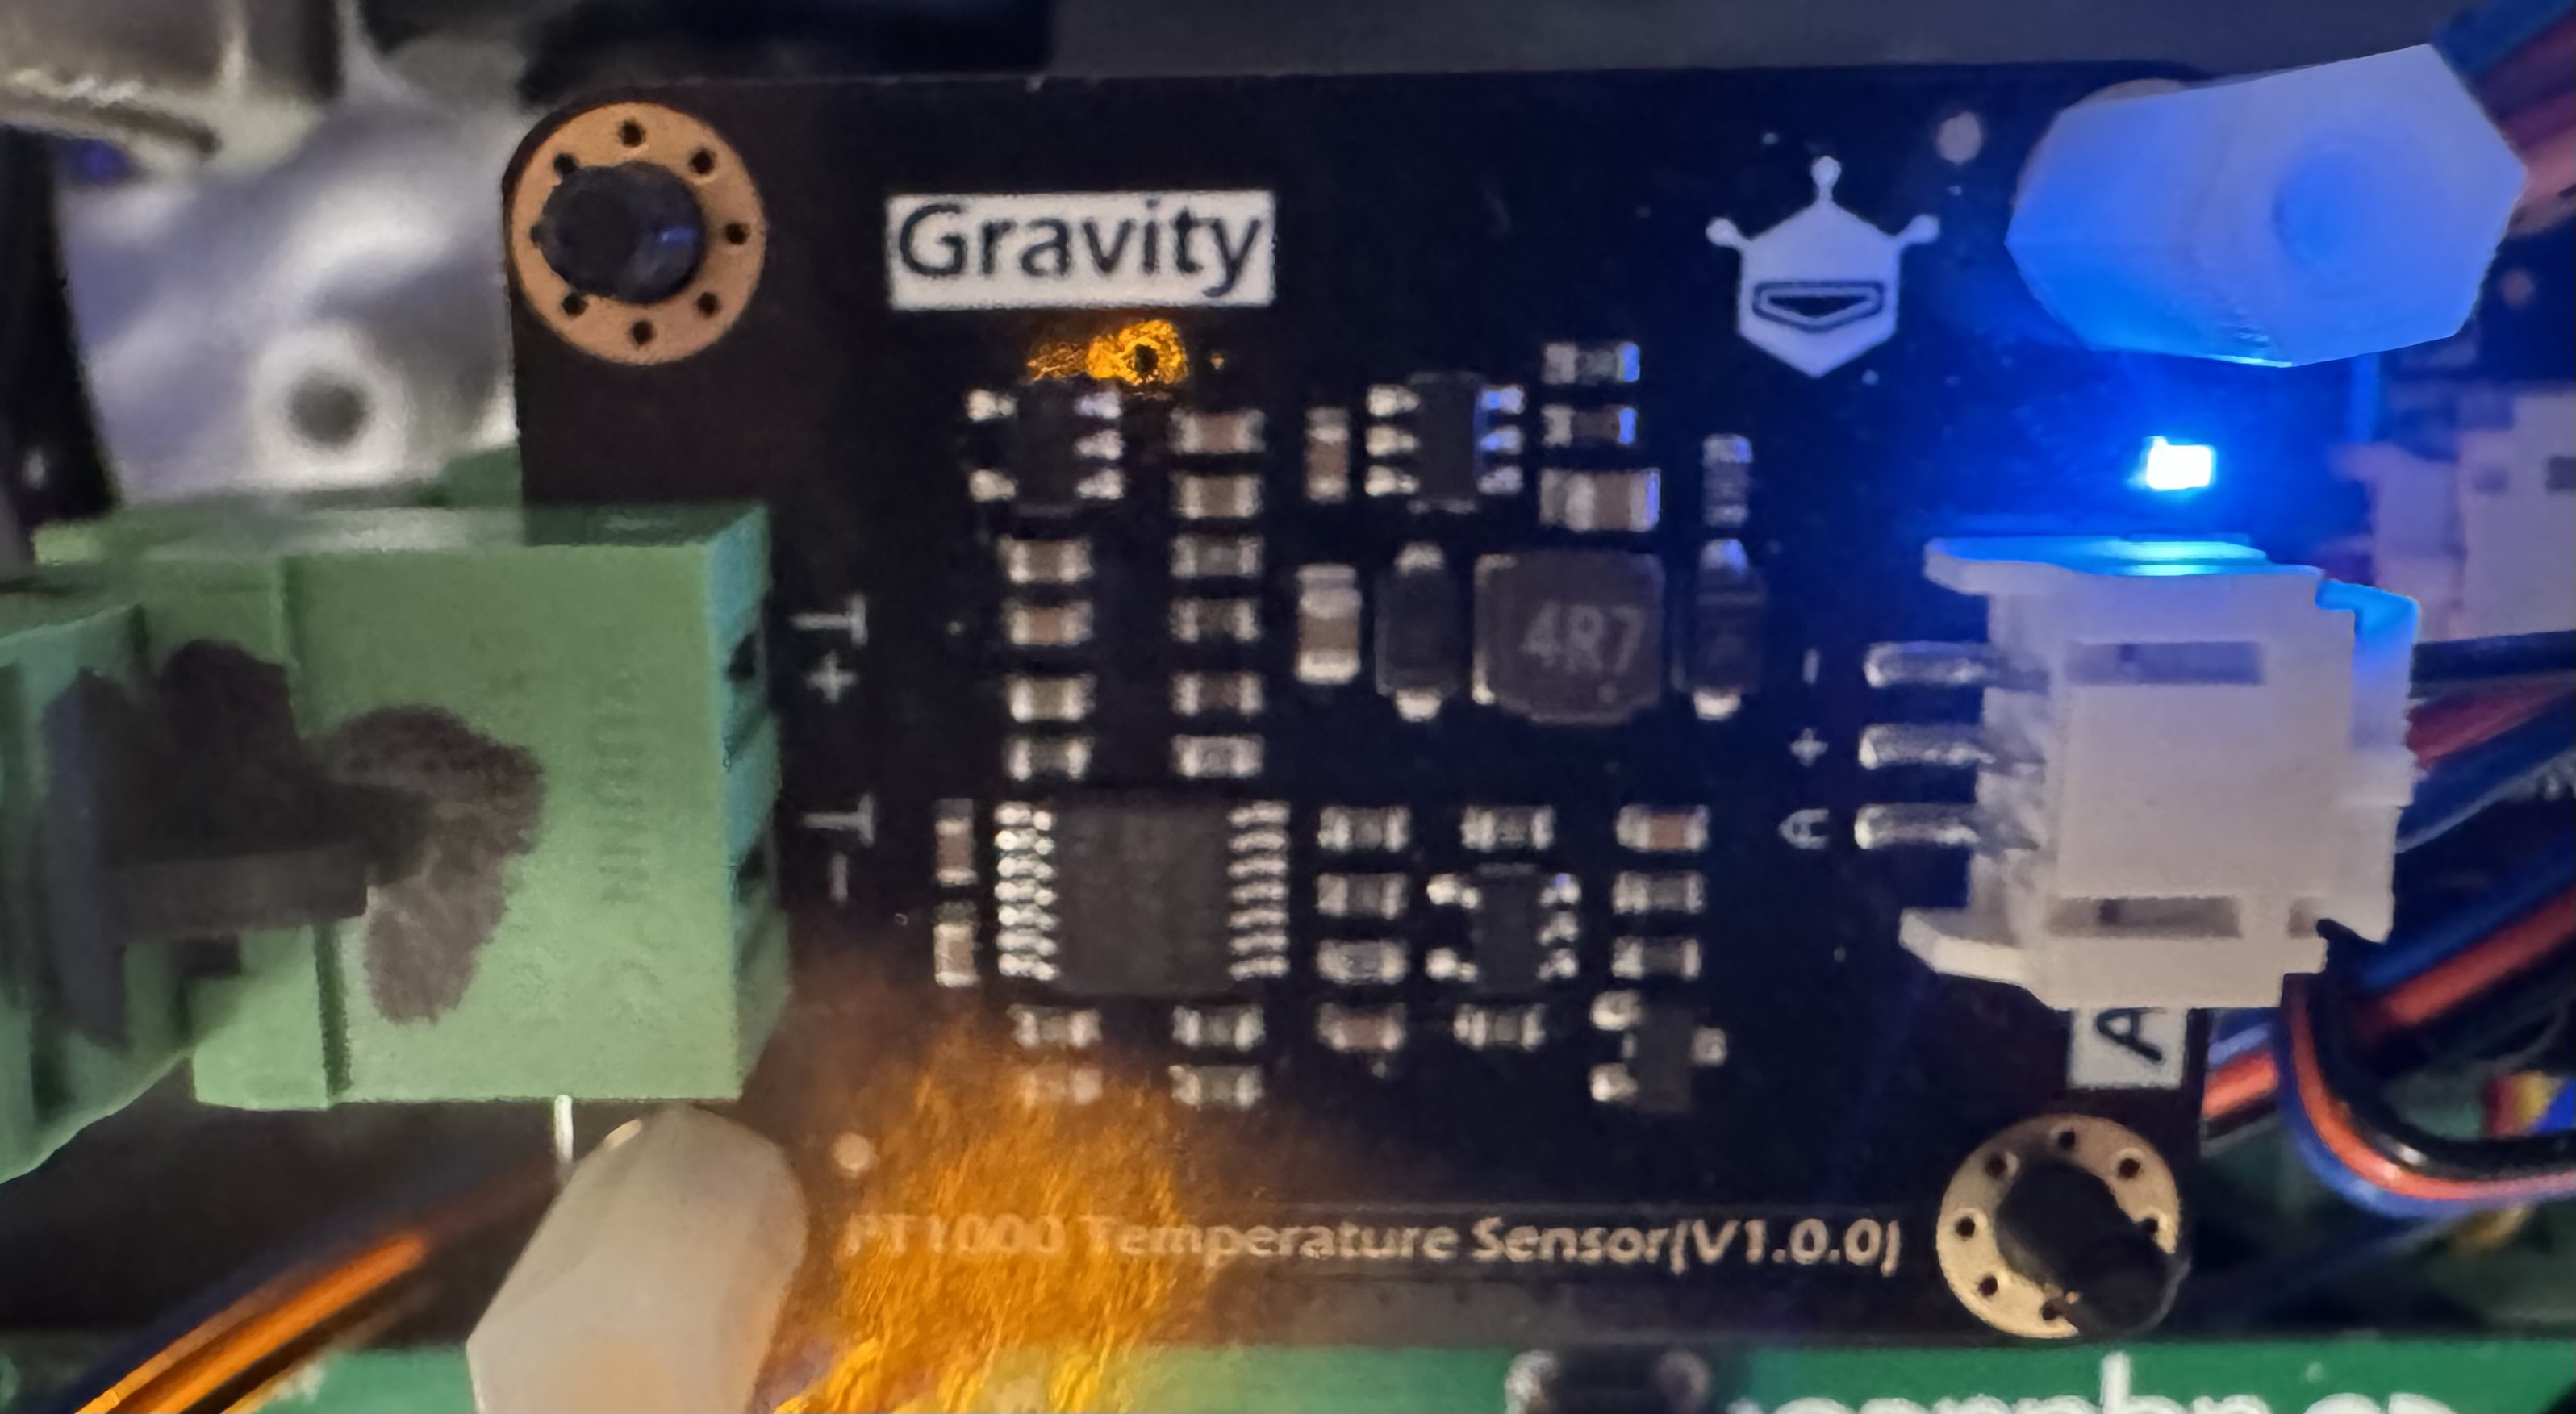
\psfig{file=Figuras/Temperature_transductor.jpeg,width=8cm,angle=0}} 
\caption{Transductor de temperatura del sensor de conductividad}\label{sensor:temp} 
\end{figure}
Los dos cables restantes, $S-$ y $S+$ (En nuestra sonda el cable S+ es tan fino que no lleva etiqueta) se conectan en la otra ficha verde, pero este sensor, el de conductividad, si tiene polaridad. De los dos transductores, que están apilados a la izquierda abajo de la caja, el superior es el correspondiente a la conductividad, (lo pone en la placa). Si se observa en el conector hembra de la ficha verde se puede ver que terminal es el positivo y cual el negativo. 
\begin{figure}[htbp!] 
\centering{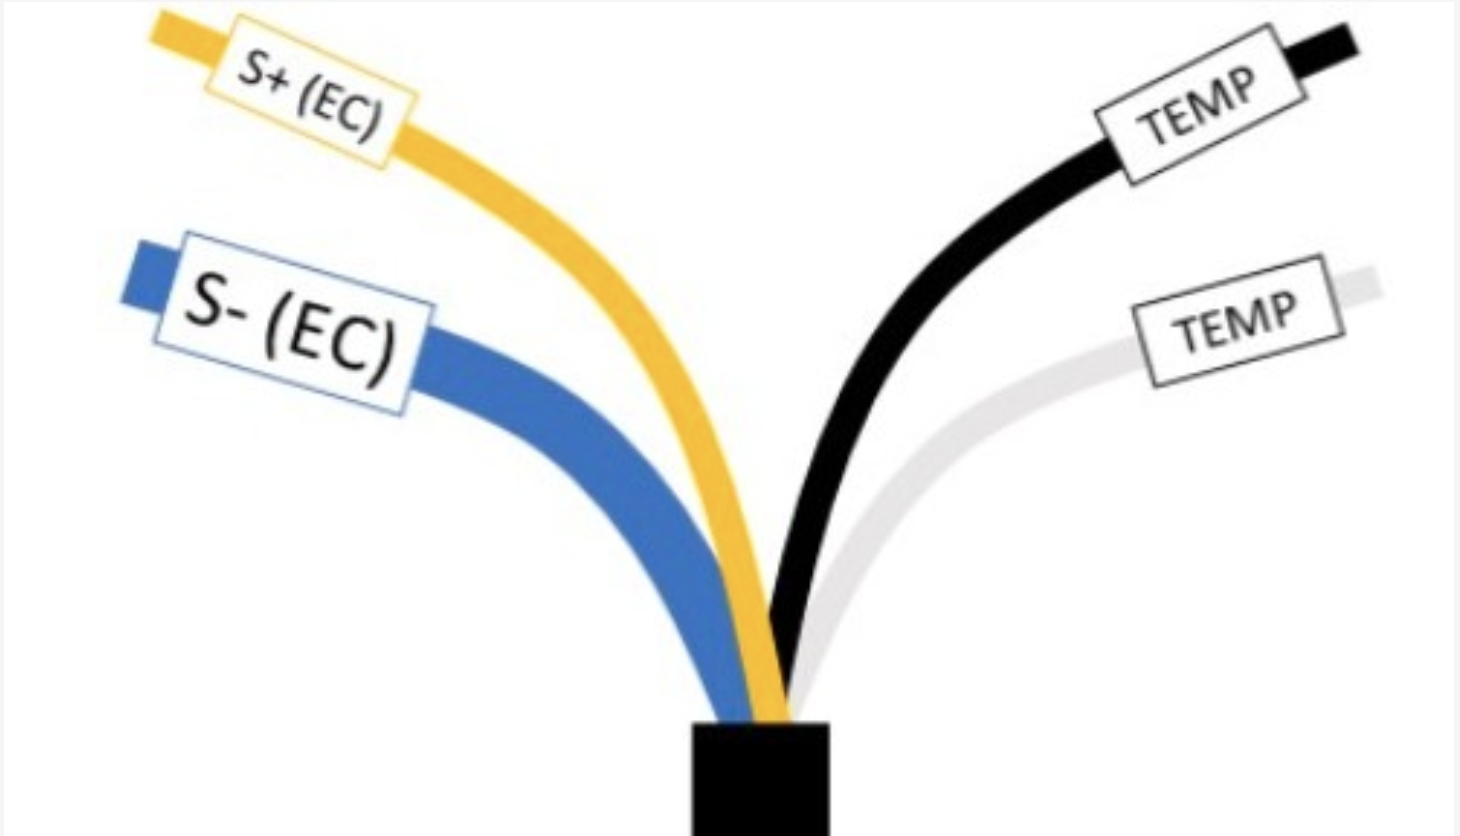
\psfig{file=Figuras/Cables_EC.png,width=6cm,angle=0}} 
\caption{Cables sonda sensor EC}\label{sensor:CEC} 
\end{figure}
\item Conectamos en el transductor superior la ficha verde correspondiente al sensor de conductividad y en la inferior en de la temperatura. Hay una tercera plaquita en el apilamiento que es otro ANALOG ISOLATOR.
\item Sacamos el cable que podamos por el prensaestopa y lo apretamos para que quede estanco.
\end{enumerate}

\end{itemize}

Los transductores de cada sensor van conectados a la placa de arriba en el lugar correspondiente:
\begin{figure}[htbp!] 
\centering{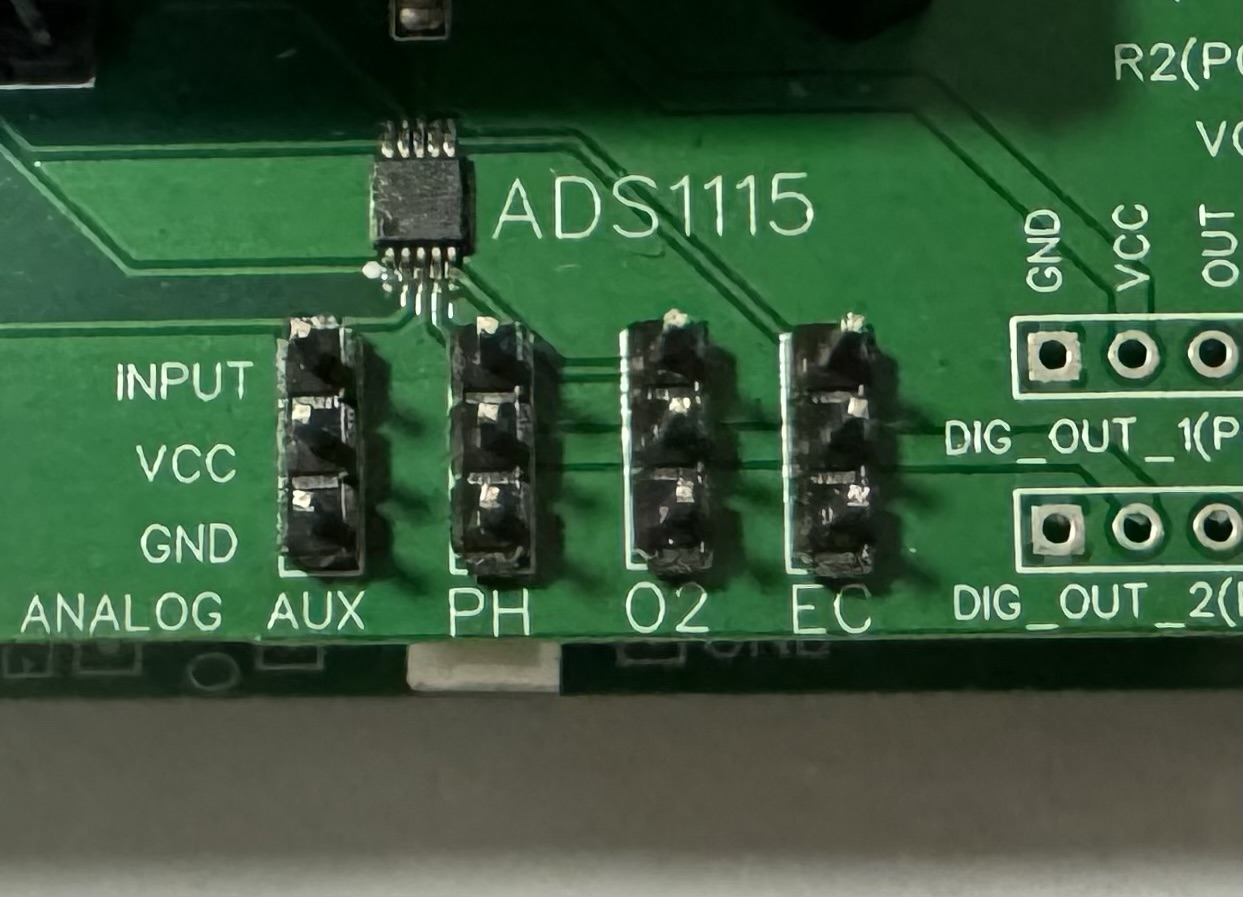
\psfig{file=Figuras/entradas_analogicas.jpeg,width=10cm,angle=0}} 
\caption{Bornes entradas analógicas}\label{sensor:Anal} 
\end{figure}
\begin{itemize}
\item El sensor de PH va conectado a los 3 pines marcados con PH. 
\item El sensor de Concentración de $O_2$ va conectado a los 3 pines marcados con O2. 
\item El sensor de Conductividad va conectado a los 3 pines marcados con EC.
\item El sensor de temperatura del la sonda de conductividad va conectado a los 3 pines marcados con AUX.
\end{itemize}

Los cables que vienen de los transductores, están compuesto por 3 hilos de los cuales uno es \underline{negro y va conectado a GND.}

\section{Puesta en marcha}

Hay que que hablar de la tarjeta micro SD y del archivo \emph{config.txt}

\begin{verbatim}
{"ssid":"MiFibra-8980","password":"nmH9Rxkt","PH1":7.3,"mV1":1715,"PH2":9.8,
"mV2":1218,"CAL1_V":256,"CAL1_T":25.75,"CAL2_V":1507,"CAL2_T":18.4,"Kec":0.9569,
"Tec":25,"mS":1413,"id":3}
\end{verbatim}

Este fichero contiene los datos de la red y los parámetros de configuración de los sensores analógicos. Veamoslo campo por campo:
\begin{itemize}
\item \textbf{"ssid":"MiFibra-8980"}. Tendrá que sustituir \emph{MiFibra-8980} por el nombre de su WIFI. Tenga en cuenta que el esp32, el micro que lleva el equipo, tiene una antena muy pequeña por lo que necesitará una señal fuerte para poder transmitir sin problemas.
\item \textbf{"password":"nmH9Rxkt"}. Tendrá que sustituir \emph{nmH9Rxkt} por el password de su WIFI.
\item \textbf{"PH1":7.3,"mV1":1715,"PH2":9.8,"mV2":1218}. Son los parámetros de configuración del sensor de PH. No los modifique, se modificarán de forma automática cuando configure dicho sensor.
\item \textbf{"\ CAL1\_V":256,"\ CAL1\_T":25.75,"\ CAL2\_V":1507,"\ CAL2\_T":18.4}. Son los parámetros de configuración del sensor de concentración de $O_2$. No los modifique, se modificarán de forma automática cuando configure dicho sensor.
\item \textbf{"Kec":0.9569,"Tec":25,"mS":1413}. Son los parámetros de configuración del sensor de concentración de Conductividad. \underline{Modifique únicamente el valor de Kec} con el valor que viene pegado en el cable de las sonda de conductividad (que es la calibración inicial, figura \ref{sensor:Kec}). Cuando pase el tiempo y el sensor necesite ser recalibrado los parámetros se modificarán de forma automática cuando configure dicho sensor.
\begin{figure}[htbp!] 
\centering{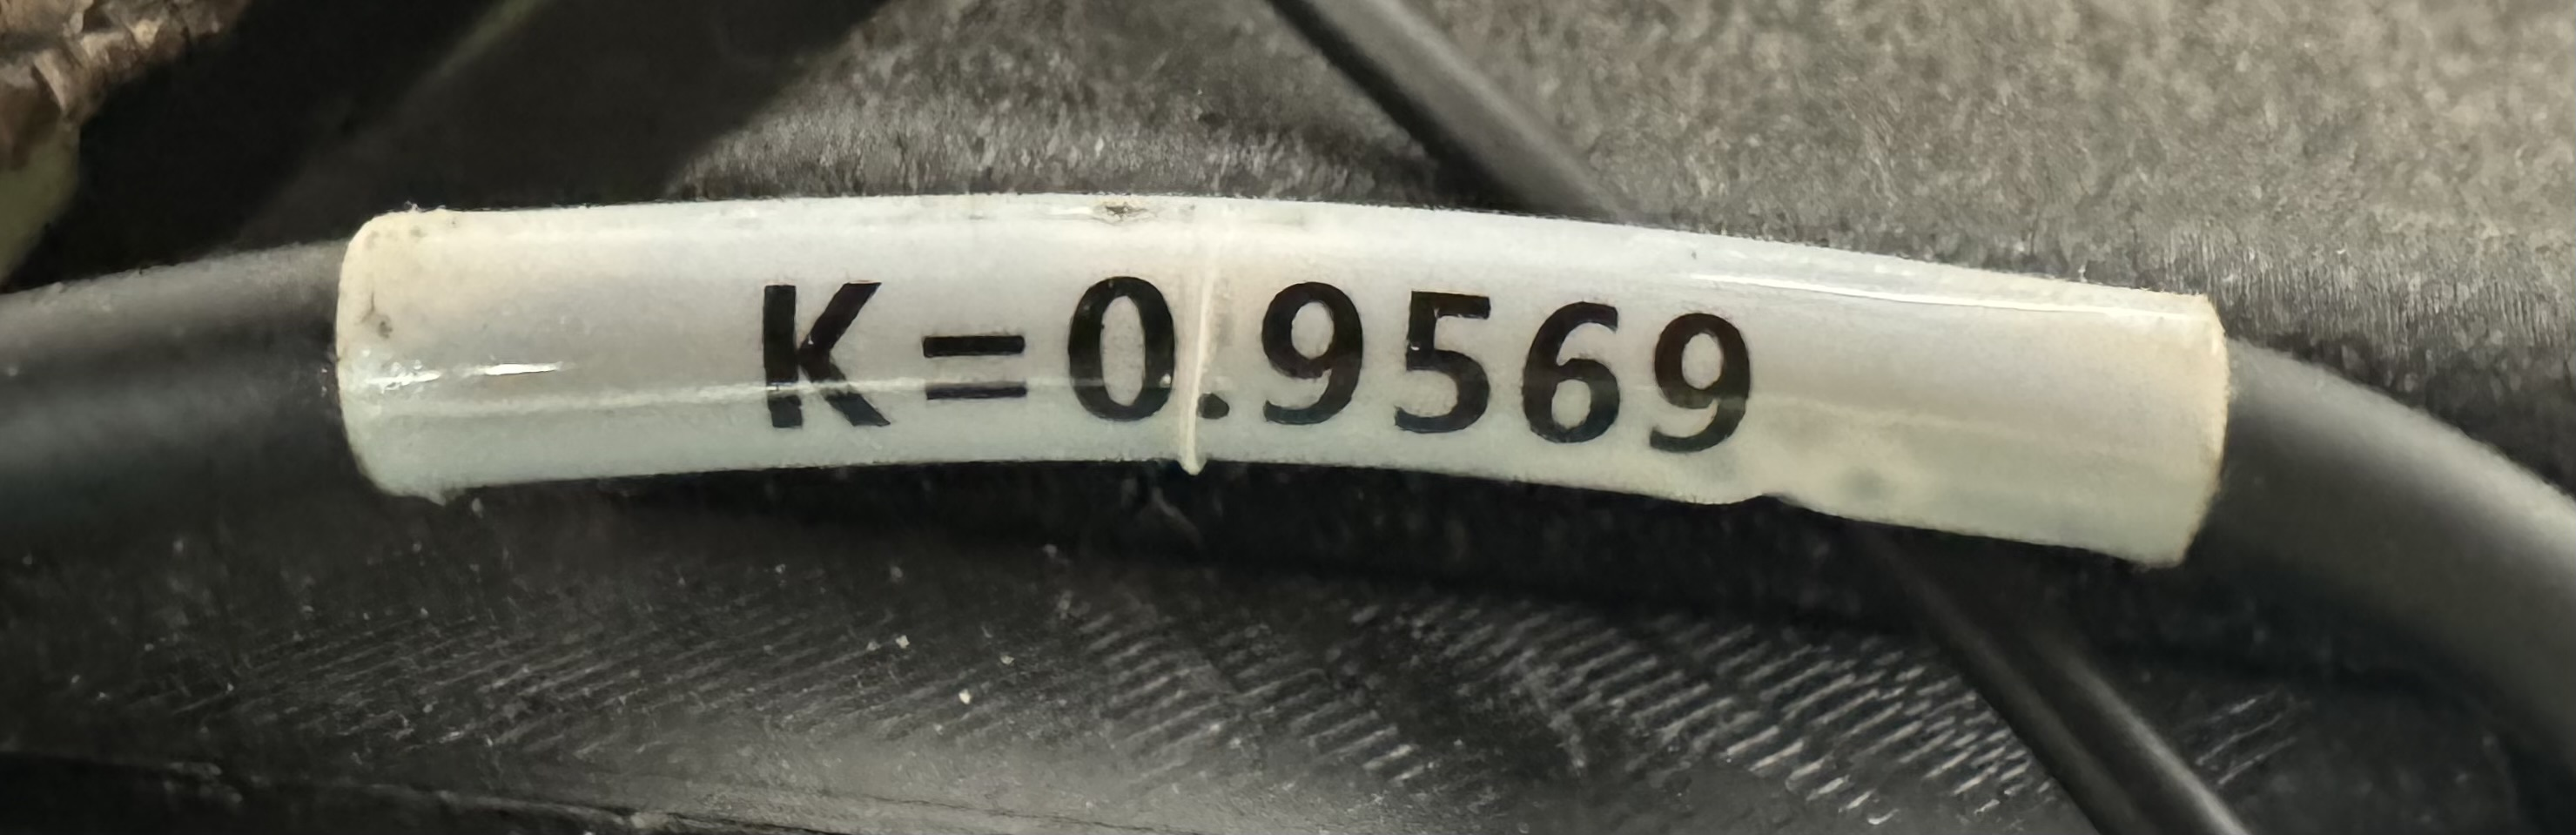
\psfig{file=Figuras/Kec.jpeg,width=6cm,angle=0}} 
\caption{Valor inicial de Kec}\label{sensor:Kec} 
\end{figure}
\item \textbf{"\ id":3}. Cada equipo tiene su propio \emph{id}. Este número determinará a que base de datos se mandan los datos recogidos. Víctor debería tener esa información.
\end{itemize}

Una vez actualizada la información , puede volver a introducir la tarjeta y en la secuencia de arranque del equipo, podría ver:
\begin{enumerate}
\item Que detecta la tarjeta microSD (se enciende el primer led de la placa superior). Si no lo hace pruebe a sacar y volver a poner la tarjeta. (Puede ver los leds en la figura \ref{botones}).
\item Que se conecta a internet, (se enciende el segundo led de la placa superior). Si no se conecta es porque no se ha puesto el nombre y la contraseña de forma correcta o porque la señal es muy débil. Pruebe a crear un punto de acceso con un móvil cerca. Configure la red en la tarjeta SD y si se conecta es por eso, tendrá que pensar como poner el router más cerca del dispositivo.
\item Una vez tenga wifi la hora del reloj se actualizará de forma automática. También se actualizará la hora del módulo de reloj interno. Este módulo mantienen la hora incluso cuando haya cortes de corriente y el aparato arranque sin covertura WIFI. Pero al menos la primera vez debe tener cobertura WIFI para que pueda actualizar la misma. Si alguna vez se perdiera la hora después de un corte de corriente , seguramente es porque se ha gastado la pila del módulo de reloj que está debajo de la placa superior del equipo. 
\item Se conecta al servidor mqtt. (se enciende el tercer led de la placa superior). Si no se conecta pero si se ha conectado a la wifi el problema debe estar en los servidores de la base de datos.
\item El cuarto led se encenderá cuando mande un dato 15 min después de que se encienda. Si durante su funcionamiento se apagase , es que no ha podido mandar el último dato. Siempre quedará una copia del mismo en la tarjeta microSD y en versiones futuras del programa se enviarán los datos que no se hallan podido mandar cuando vuelva a haber cobertura wifi.
\end{enumerate}

